\documentclass[a4paper,12pt]{jarticle}
\input ./chap01_preamble.tex
\graphicspath{%
  {../text01-img/}%
}
% !TEX root = ./chap01_05.tex
\begin{document}
\section{でんげんの切り方を覚えよう}
\ \ 皆さんのデータはmicroSDカードに保存されています。
でんげんを急に切るとmicroSDカードに書き込まれる前に本体のでんげんが切れてしまいまい、
データが壊れたりする可能性があります。

そこで、でんげんを切る際は、決められた手順に従う必要があります。
この節ではでんげんの切り方を学びます。
ラズベリーパイを使い終わったら正しい手順ででんげんが切れるように覚えておきましょう。



\centering
\begin{minipage}{8.115cm}
  {\upshape
    \centering
    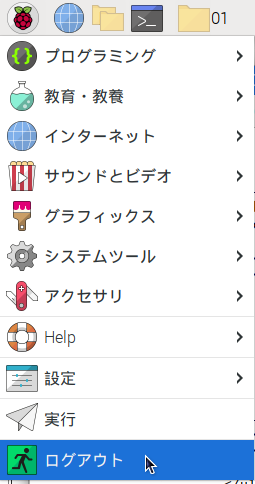
\includegraphics[width=2.1cm,height=5.1cm]{textbook-img206.png}
    \newline
    Figure {\refstepcounter{Figure}\theFigure\label{seq:refFigure40}}: 「ログアウト」メニュー}
\end{minipage}
\begin{minipage}{7.115cm}
  Figure~\ref{seq:refFigure40}のようにラズベリーのアイコンをクリックすると一番下に「ログアウト」があります。
  これをクリックしてください。
\end{minipage}
\bigskip


\flushleft
\textcolor[rgb]{0.13333334,0.13333334,0.13333334}{Figure~\ref{seq:refFigure42}のような画面となったら一番上の「Shutdown」を押してでんげんを切ります。}
\bigskip
\centering
\begin{minipage}{8.225cm}
  {\upshape
    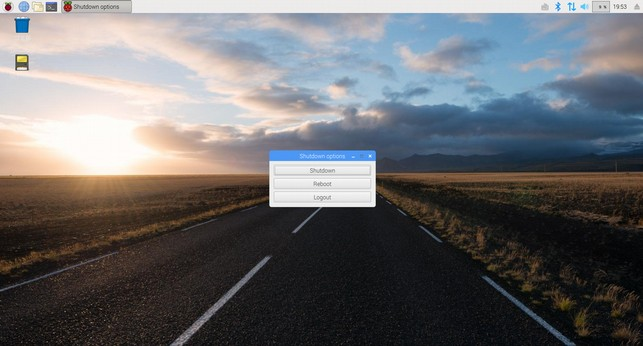
\includegraphics[width=8.1cm,height=4.5cm]{textbook-img208.jpg}
    Figure {\refstepcounter{Figure}\theFigure\label{seq:refFigure42}}: 「Shutdown」画面}
\end{minipage}

\bigskip
\flushleft
\textcolor[rgb]{0.13333334,0.13333334,0.13333334}{ラズベリーパイ本体の緑色のランプが消灯します。
  Figure~\ref{seq:refFigure41}。
  この状態になったらでんげんアダプターをコンセントから抜きましょう。}

\bigskip
\centering
\begin{minipage}{8.207cm}
  {\upshape
    \includegraphics[height=4.5cm]{textbook-img207-2023.png}
    \newline
    Figure {\refstepcounter{Figure}\theFigure\label{seq:refFigure41}}: Raspberry Pi
    ステータスランプ}
\end{minipage}
\clearpage\subsection{安全な持ち帰り方}
\flushleft
\ \ ラズベリーパイなどの電子機器はらんぼうに扱うと壊れてしまいます。また、静電気にも弱いです。ラズベリーパイを持ち帰るときはラズベリーパイを付属の袋と箱へ入れて持ち帰りましょう。この袋は静電気を防いでくれます。microSDカードはなくさないようにラズベリーパイに挿しておきましょう。

\clearpage
\end{document}